\documentclass[border=7pt]{standalone}
\usepackage{amsmath,amssymb,bm,mathtools}
\usepackage[fontset=none]{ctex}
\setCJKmainfont{Songti SC}\setCJKsansfont{PingFang SC}
\usepackage{tikz}\usetikzlibrary{arrows.meta,calc,patterns,angles,quotes,decorations.markings,decorations.pathmorphing}
\newcommand{\dd}{\mathop{}\!\mathrm d}
\definecolor{blue}{HTML}{235789}\definecolor{red}{HTML}{BC4B41}
\tikzset{axis/.style={->,>=Stealth,line width=.55pt},world/.style={line width=.9pt},flow/.style={->,>=Stealth,line width=.85pt},ray/.style={->,>=Stealth,line width=.85pt},guide/.style={dashed,line width=.4pt},aux/.style={dashed,line width=.4pt},dim/.style={<->,>=Stealth,line width=.5pt},every node/.style={font=\normalsize},force/.style={->,>=Stealth,very thick},gas/.style={fill=blue!7}}
\begin{document}
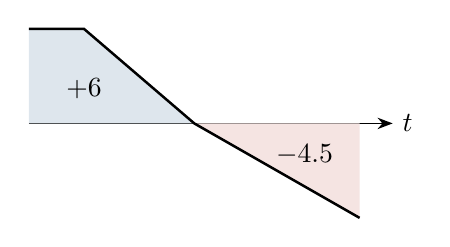
\begin{tikzpicture}\begin{scope}[x=.7cm,y=.4cm]\draw[axis](0,0)--(6.6,0)node[right]{$t$};\fill[blue!15](0,0)--(0,3)--(1,3)--(3,0)--cycle;\fill[red!15](3,0)--(6,-3)--(6,0)--cycle;\draw[world](0,3)--(1,3)--(3,0)--(6,-3);\node at(1,1.1){$+6$};\node at(5,-1){$-4.5$};\end{scope}\end{tikzpicture}
\end{document}
